\documentclass[../main/report.tex]{subfiles}
\begin{document}

\chapter{PCB}
\label{sec:pcb}

This chapter will describe the PCB layout, the main components and the design philosophy that went into solving the system requirements.
%\section{Layout Overview}
\section{Physical system structure}

\missingfigure{Physical overview}


\section{Design for Redundancy}

When designing a PCB for a system, there is no easy way to correct mistakes.
A wire can not be rerouted if there is a problem.
Because of this, a lot of effort has gone into making backup plans if something fails.
Each part of the PCB needs to be able to work without the rest of the PCB.
This is done by having jumpers on each section, which can be rerouted manually.
That way each part can be connected to other parts of the board, or to other sources.
Because of this, the board is not optimized for size, but was rather made to optimize for highest possible chance of success.

This small graphics explains the design philosophy of the PCB
\begin{verbatim}
     -----------------
    | Backup solution |
    |                 |
    |  -------------  |
    | | Core design | |
    | |             | |
    | |             | |
    | --------------- |
    |                 |
     -----------------
\end{verbatim}

\section{Main Components}

\subsection{Microcontroller / System Control Unit}
The EFM32 Giant Gecko 32-bit Microcontroller from Energy Micro was chosen as the controller for this project.
A microcontroller from Energy Micro was required for the task and this particular controller is
very energy efficient, which is a plus.
In addition to this, there were a lot of development boards available,
plus over half of the group had experience with this controller from the subject
TDT4258 Energy Efficient Computer Systems.

The EFM32GG990F512-BGA112 was chosen as a powerful enough version of the microcontroller.

\subsection{FPGA}
The XC6SLX45-2CSG324I FPGA of the Spartan-6 family from Xilinx was chosen as the FPGA.
This particular FPGA has been used for different tasks on the university before, and the support systems are therefore available to us.
The version was the one used on the PCB.
A less powerful version of this one was available for testing on development boards in the lab.

\section{Input}

The main source of data communication between microcontroller and a host PC is USB.
This protocol has been used for years on projects like these, with good results. \todo{citation needed}

However, if the USB fails, there are backup plans.
Primarily a serial port (RS-232) has been included to work if the USB should fail.
If this also fails, the wires from the serial port is put on headers, which can be used as GPIO pins.

\section{Output}
The main source of output from the FPGA is an HDMI connector.
This is a novel feature this year, as no previous group has tried to implement it before.

Because of this new challenge, a lot of backup schemes were put in place.
The HDMI connector is put on headers, in case the connector fails.
A separate VGA module is connected to the FPGA, in case the HDMI doesn't work and if this fails, a VGA module is also connected to the microcontroller.

\section{Power}

The system is powered by a 5V mini usb. The core design is implemented such that this connection feeds electricity towards two voltage regulator circuits. These, in turn power up the rest of the machine. The usb connection has a backup solution in the form of a header through which the 5V line must pass immediately after entering the pcb. This is done so that the incoming electricity can easily be probed for voltage level and also so that in case the usb connection fails, an external power supply can be connected to the board.

\begin{figure}[H]
		\centering
		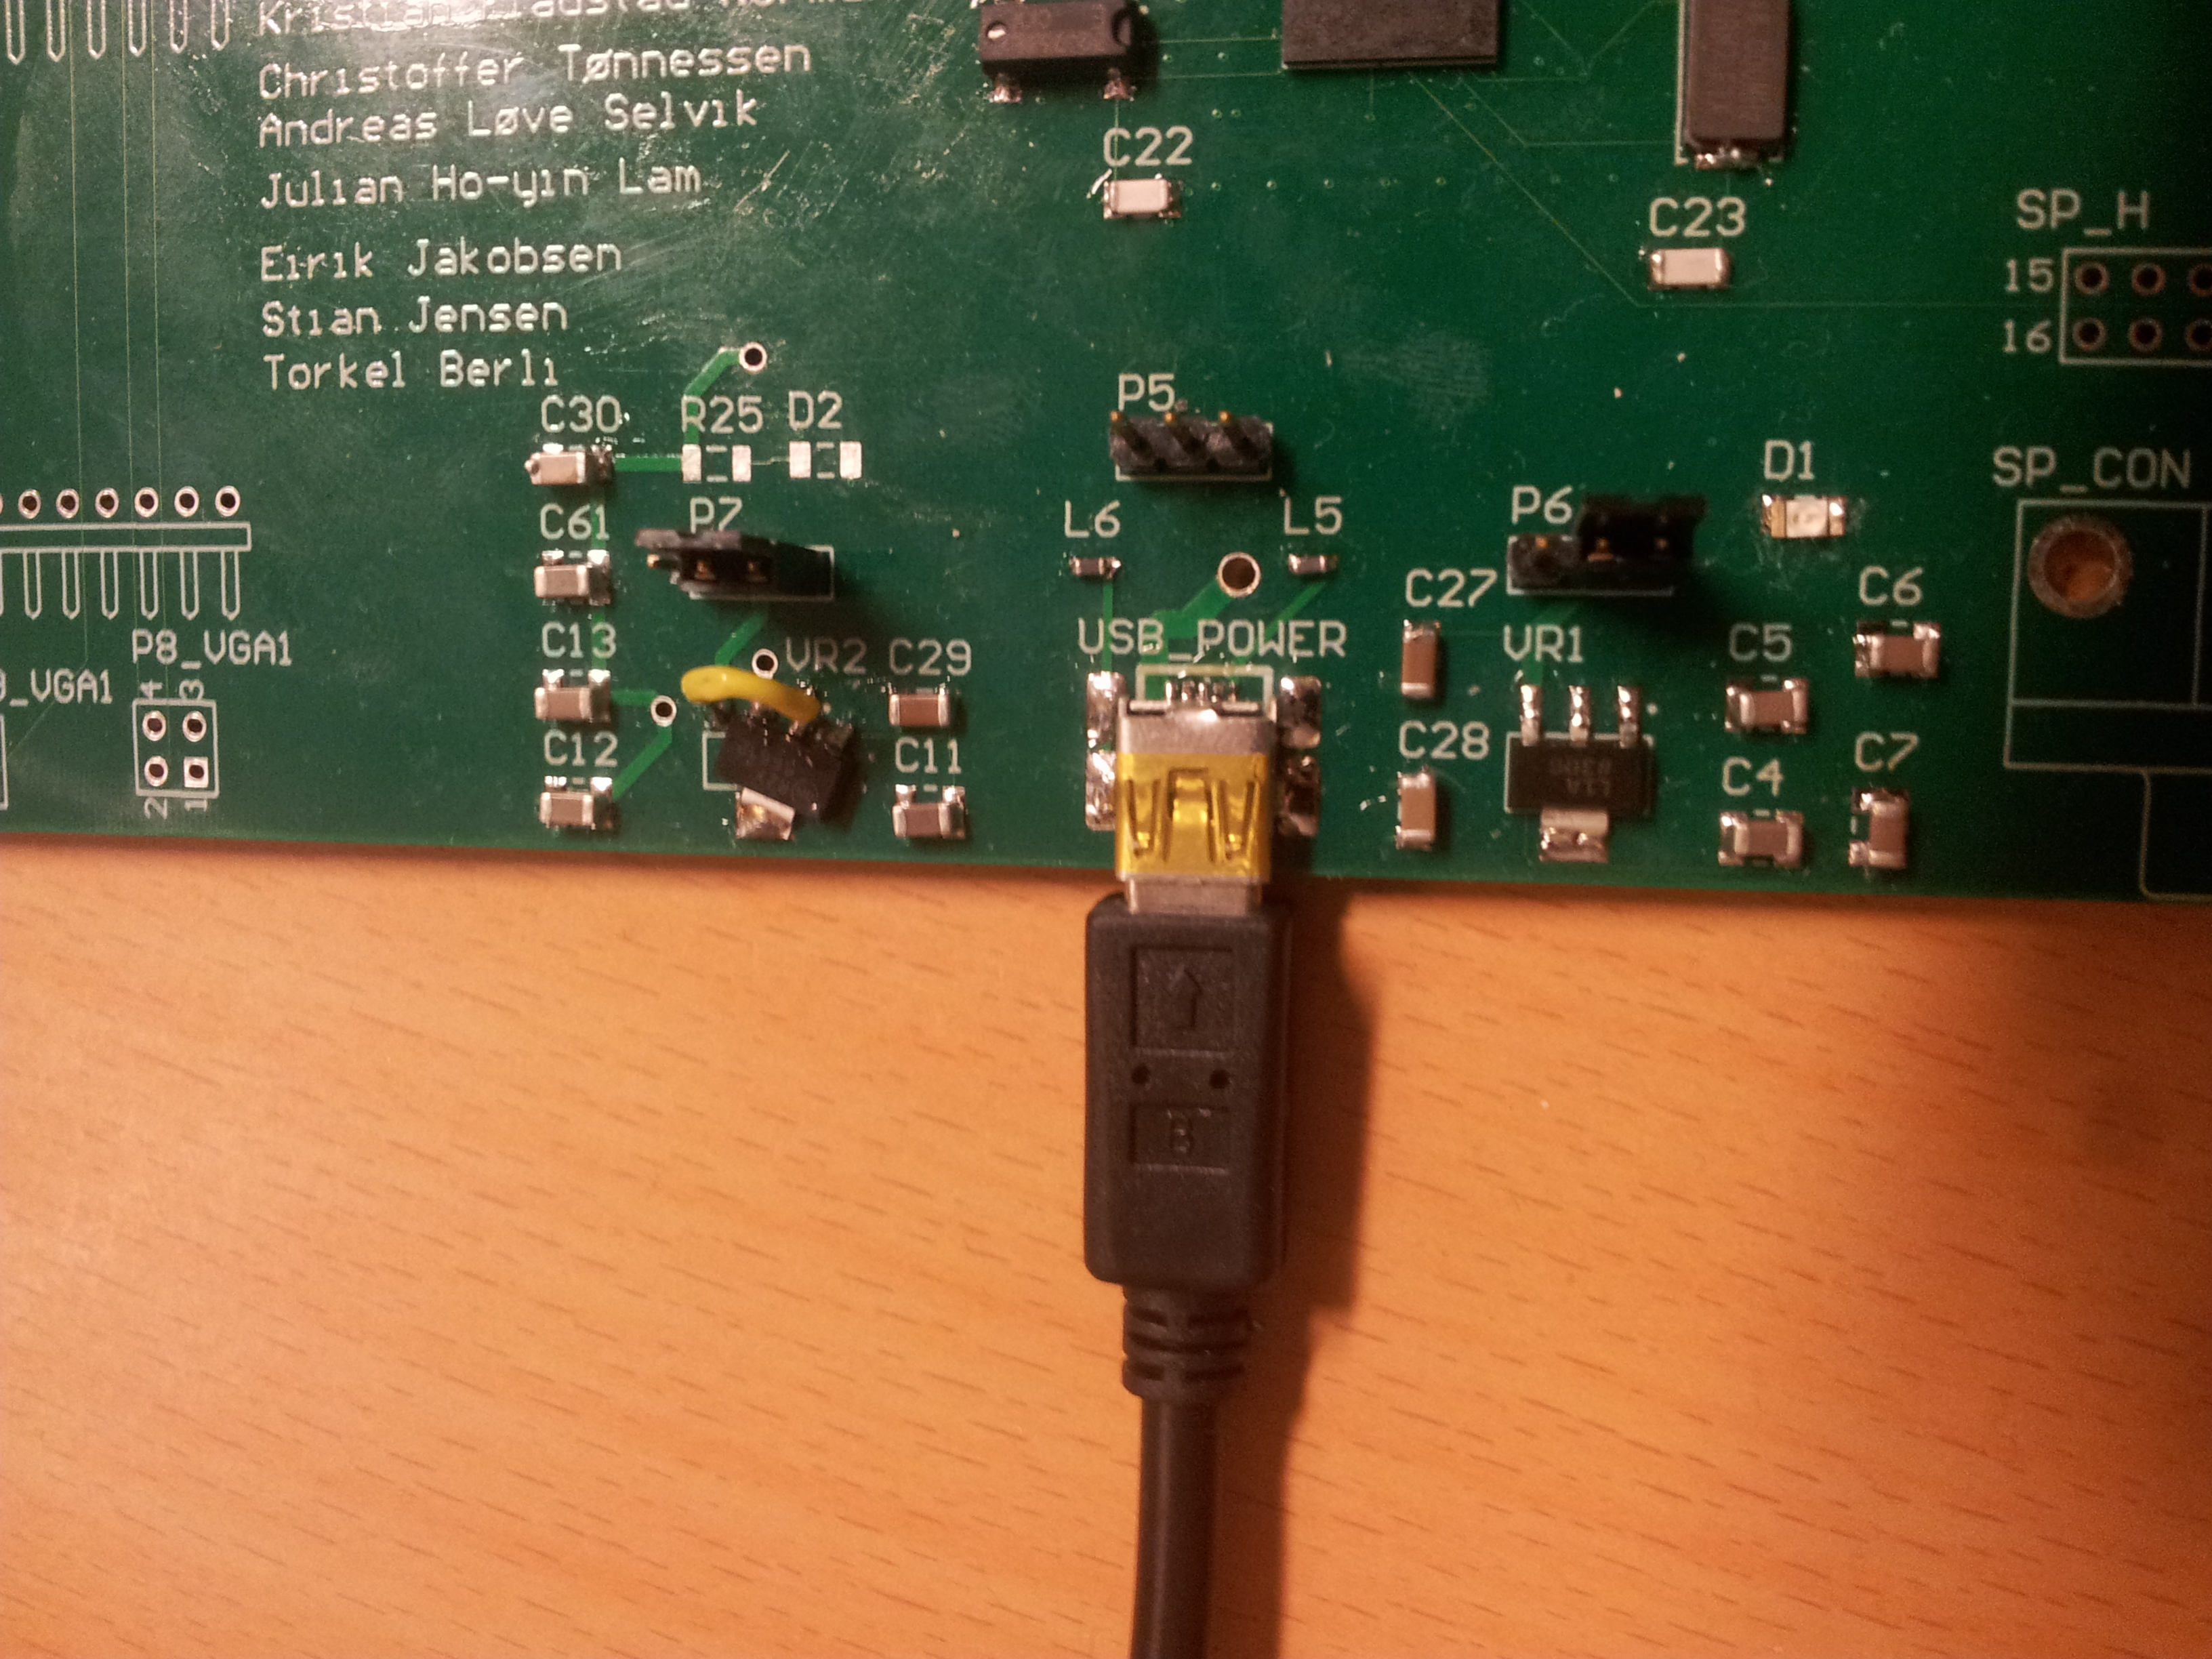
\includegraphics[width=0.65\textwidth]{../pcb/assets/power.jpg}
		\caption{Picture of physical power circuit}
		\label{fig: power picture}
\end{figure}

\section{Bus}
Standard EBI connection between FPGA and MCU, but with headers in between such that external connection can be done in case of failure on one side of the connection, as well as an easy way to check transmitted signals during debugging.

\section{Clocks}
FPGA oscillator along with header on which an external oscillator resource can be connected by way of backup.
The microcontroller clocks on the other hand have a backup solution in that the microcontroller has internal RC-oscillators for use in case the crystals malfunction.


\section{Footprints}
Predominantly SMDs(surface mounted device) large enough for humans to solder(with a couple of exceptions)

\subfile{../pcb/hdmi.tex}

\todo{...Uncertain ie om at vi endra litt på en del footprints, men pga hvordan fysiske komponenter funker,}

\subsubsection{Prebundled}

\subsubsection{Handmade}
Some footprints we had to make ourselves.
This was done inside Altium.
The specification for the footprints was found in the datasheets of the component in question.

When making the handmade footprints some other thoughts were taken into account.

\begin{itemize}
    \item We need to solder these components
    \item The connection on the components is physical, as long as it leads current, it will work.
    \item Some datasheets didn't match the component exactly, but was for a sister component
\end{itemize}

With this in mind we made footprints which was slightly bigger than it needed to.

\begin{verbatim}
Needed:                 Actual:
--------------          --------------
|            |          |            |
|--|      |--|       |--|--|      |--|--|
|  |      |  |       |  |  |      |  |  |
|..|      |--|       |--|..|      |--|--|
|            |          |            |
--------------          --------------
\end{verbatim}
\end{document}
